\documentclass[../../main.tex]{subfiles}

\begin{document}

\subsection{Cloud computing}
Je to technológia, ktorá dodáva cez internet počítačové služby zahŕňajúce servery, dátové úložiská, databázy, počítačové siete, softvér, analýzu...Technológia ponúka flexibilné zdroje, inovácie a úspory dosiahnutím škálovatelnosti. Zákazník platí len za služby, ktoré využíva. Pomocou tejto technológie je možné tvoriť aplikácie finančne úspornejšie, využívať a meniť zloženie stroja, aby som dosiahol len potrebné množstvo, ktoré sa bude využívať, zlepšenie výkonu, bezpečnosti, rýchlosti, produktivity a odolnosti.
Cloudové služby môžu byť nasadené na verejnom, privátnom alebo hybridnom cloude.
\begin{description}
    \item[Verejný cloud:] je vlastnený a ovládaný treťou stranou, ktorou je cloudový prevádzkovateľ, ktorý dodáva zdroje cez internet. Všetok hardvér aj softvér patrí tomuto prevádzkovateľovi. Klient pristupuje k týmto službám cez webový prehliadač.
    \item[Privátny cloud:] sa skladá zo zdrojov, ktoré patria exkluzívne jednej spoločnosti. Môže byť priamo umiestnený v dátovom centre spoločnosti. Používa privátnu sieť.
    \item[Hybridný cloud:] je kombinácia privátneho a verejného cloudu. Môžu si medzi sebou presúvať aplikácie čím je možné dosiahnuť nové možnosti. 
\end{description}

Služby Cloud computing spadajú do 4 kategórií:
\begin{description}
     \item[Infrastructure as a service (IaaS)] je najčastejšia kategória služieb. Ide o prenájom serverov, virtuálnych strojov, dátových úložísk, sietí a operačných systémov od cloudového prevádzkovateľa.
     \item[Platform as a service (PaaS)] je služba na dopyt, ktorá je dodávaná s prostredím  pre vývoj, testovanie a manažovanie softvérových aplikácií. Umožňuje rýchlejší vývoj aplikácií.
     \item[Serverless computing] zameriava sa na budovanie aplikácií bez manažovania serverov a potrebnej infraštruktúry. Cloudový prevádzkovateľ sa stará o nastavenie, kapacitu a manažovanie servera pre klienta.
     \item[Software as a service (SaaS)] je metóda pre dodávanie aplikácií cez internet, väčšinou cez predplatné. Cloudový prevádzkovateľ udržiava aplikáciu a jej infraštruktúru. vykonáva aj aktualizáciu softvéru.\cite{azure_cloud}
\end{description}

 \begin{figure}[h!]
 \centering
  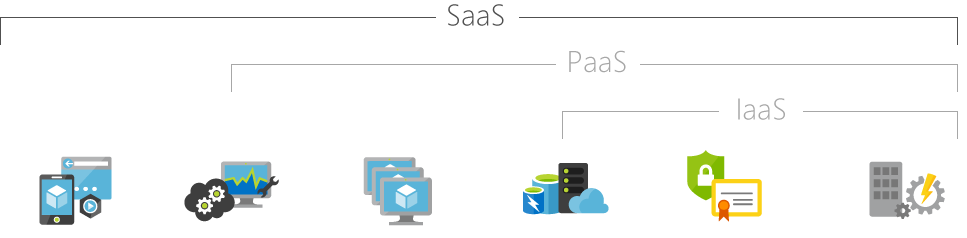
\includegraphics[scale=0.5]{images/azure_services.png}
  \caption{Cloud computing - služby\cite{azure_cloud}}
    \label{fig:azure_services}
\end{figure} 

\subfile{sections/Cloud_computing/azure_popis.tex}

\end{document}


% doplniť cloudivych prevadzkovatelov

